% !TeX root = ../main.tex

\section{Introduzione}
La continua crescita della quantità di dispositivi mobile in circolazione ha reso molto importante a livello globale il mercato delle applicazioni mobile e per questo motivo sono sempre di più le aziende che decidono di investire risorse nello sviluppo e nella vendita di applicazioni mobile. 
Una azienda che intende puntare al maggior numero di utenti possibile con le proprie applicazioni deve considerare che l'intero mercato è spartito in base alla diffusione dei sistemi operativi per dispositivi mobile. 

Ad oggi, 
i sistemi operativi più diffusi sono Android (Google) e iOS (Apple), 
i quali coprono quasi la totalità del mercato con quote rispettivamente del 71\% e del 28\%\footnote{\href{https://www.statista.com/statistics/272698/global-market-share-held-by-mobile-operating-systems-since-2009/}{https://www.statista.com/statistics/272698/global-market-share-held-by-mobile-operating-systems-since-2009/}}.
Questi dati comportano per un'azienda la necessità di sviluppare la stessa applicazione per almeno due piattaforme completamente differenti tra loro. 
A tal proposito sono nate nuove metodologie e tecniche basate sul concetto ``\textit{Write Once, Run Anywhere}''\footnote{\href{https://www.computerweekly.com/feature/Write-once-run-anywhere}{https://www.computerweekly.com/feature/Write-once-run-anywhere}} (WORA) con lo scopo di ottimizzare lo sviluppo delle applicazioni mobile al fine di ridurre i costi e aumentare l'efficienza del processo di sviluppo.

Le principali tecniche moderne di sviluppo per applicazioni mobile che seguono questi concetti sono:
\begin{itemize}
    \item \textbf{Cross-platform} - Rispetta completamente la filosofia WORA. Lo stesso codice può essere eseguito su diverse piattaforme grazie ad uno strato applicativo aggiuntivo che si occupa di interpretare il codice e tradurlo nel linguaggio specifico della piattaforma target.
    
    \item \textbf{Multi-platform} - Tecnica più recente che permette di sviluppare applicazioni native condividendo solamente la logica applicativa. In questo caso non è necessario uno strato software aggiuntivo perché l'applicazione può essere eseguita direttamente dalla piattaforma target.
\end{itemize}

\section{Cross-platform vs Multi-platform}
Sia nel caso cross-platform che nel caso multi-platform i principali vantaggi,
che sono la riduzione dei costi e l'ottimizzazione del processo di sviluppo, 
derivano dalla condivisione e dal riuso del codice e quindi meno risorse impiegate rispetto allo sviluppo classico delle applicazioni mobile native.

Esistono però alcune differenze tra loro,
fondamentali durante la scelta della metodologia da adottare da parte di un'azienda per lo sviluppo di una applicazione mobile.

\begin{itemize}
    \item \textbf{Cross-platform}
    \begin{itemize}
        \item Condivisione/riuso totale del codice. Sia la logica applicativa che l'interfaccia utente sono le stesse per qualsiasi piattaforma.
        
        \item Performance limitate rispetto al nativo, dovute alla presenza di uno strato software aggiuntivo che interpreta e traduce il codice.
        
        \item Accesso alle funzionalità hardware del dispositivo limitato e/o con overhead, dovuto sempre alla presenza dello strato software aggiuntivo.
    \end{itemize}
    
    \item \textbf{Multi-platform}
    \begin{itemize}
        \item Condivisione/riuso della sola logica applicativa. Lo sviluppo dell'interfaccia utente rimane nativo.
        
        \item Performance elevate, equivalenti a quelle native.
        
        \item Accesso completo e senza overhead a tutte le funzionalità hardware del dispositivo.
    \end{itemize}
\end{itemize}

\section{Strumenti}
\label{app-multiplatform-tools}
La scelta degli strumenti da utilizzare nel processo di sviluppo è influenzata da tantissimi fattori come ad esempio la necessità di una licenza commerciale, 
i gusti dello sviluppatore e certamente le tecnologie coinvolte. 
A prescindere da questi fattori,
è possibile definire delle categorie di strumenti, 
utilizzati per qualsiasi tipologia di software: 
(\textit{i}) linguaggio di programmazione, 
(\textit{ii}) ambiente di sviluppo (IDE\footnote{Integrated Development Environment}), 
(\textit{iii}) build automation, 
(\textit{iv}) distribuzione software e (\textit{v}) framework di sviluppo.

Un altro fattore che vincola la scelta degli strumenti è la piattaforma target,
ovvero l'ambiente dove eseguirà il codice,
e lo è in particolare per le applicazioni mobile. 
A differenza dello sviluppo di applicazioni Android,
dove gran parte degli strumenti più diffusi è open-source, 
lo sviluppo di applicazioni iOS è soggetto a vincoli stringenti imposti da Apple: 
tutta la toolchain necessaria è disponibile solamente per il sistema operativo macOS.

\subsection*{Linguaggio di programmazione}
Una moderna applicazione nativa per iOS è sviluppata in codice \textit{Swift}\footnote{\href{https://www.swift.org/}{https://www.swift.org/}}, 
un linguaggio di programmazione open-source progettato da Apple e realizzato per sostituire il linguaggio Objective-C~\cite{kerr2018beginning}.

Come nel caso delle applicazioni iOS,
anche per quelle Android è stato adottato un nuovo linguaggio per sostituire quello precedentemente utilizzato. 
Il linguaggio di programmazione ufficiale per lo sviluppo di applicazioni Android è il linguaggio open-source creato da JetBrains chiamato \textit{Kotlin}\footnote{\href{https://kotlinlang.org/}{https://kotlinlang.org/}}. 
Questo linguaggio ha sostituito Java grazie alla sua interoperabilità con quest'ultimo: 
il codice Kotlin può infatti essere compilato in bytecode Java e quindi essere eseguito ovunque può eseguire una JVM\footnote{Java Virtual Machine}~\cite{laurence2021programming}.

\subsection*{Ambiente di sviluppo}
L'ambiente di sviluppo consiste in un programma software a supporto dello sviluppatore per la fase di scrittura del codice. 
Un IDE consiste di più componenti: 
oltre all'editor principale infatti solitamente comprende tool di build automation, 
debugger, 
compilatore/interprete e emulatori.

Per poter sviluppare ed eseguire un'applicazione iOS,
l'unico IDE stabile è \textit{XCode}, 
disponibile solamente per macOS. 
Per lo sviluppo di applicazioni Android invece esistono diversi IDE ma sicuramente quello più diffuso è \textit{Android Studio}:
un'ambiente di sviluppo open-source costruito sul robusto e popolare IntelliJ di JetBrains,
distribuito con tutte le funzionalità necessarie per lo sviluppo Android già preinstallate.

\subsection*{Build automation}
Con \textit{Build Automation} si intende l'automazione di alcuni task del processo di sviluppo come la compilazione del codice, 
l'esecuzione dei test, 
la firma del codice e la pacchettizzazione. 
Gli strumenti di build automation sono nati dunque per supportare lo sviluppatore permettendogli di automatizzare operazioni semplici e ripetibili. 
Tipicamente un task viene descritto per il raggiungimento di un \textit{goal} tramite un elenco ordinato di sotto-task dipendenti tra loro.

La build automation per lo sviluppo di applicazioni Android è supportata dal tool \textit{Gradle}\footnote{\href{https://gradle.org/}{https://gradle.org/}}, 
uno strumento open-source per build automation e dependency management. 
Gradle fornisce il proprio DSL\footnote{Domain Specific Language}, 
disponibile sia in Groovy che Kotlin, 
per la definizione degli script di build~\cite{nagy2022simplifying}.

In ambiente Apple è necessario installare il pacchetto \textit{Command Line Tools for XCode}, il quale contiene un insieme di strumenti di sviluppo tra cui \textit{Swift Package Manager}, dedicato alla build automation e alla dependency management. Anche se disponibile tra le funzionalità del tool ufficiale Apple, la gestione delle dipendenze tipicamente viene svolta tramite un altro strumento molto diffuso chiamato \textit{CocoaPods}\footnote{\href{https://cocoapods.org/}{https://cocoapods.org/}}.

\subsection*{Distribuzione software}
In questo caso è più corretto parlare di servizi di distribuzione software invece che di strumenti. 
Gli strumenti utilizzati dallo sviluppatore corrispondono infatti a quelli di build automation con lo scopo di firmare ed effettuare l'upload dell'applicazione su una piattaforma apposita per la distribuzione. 
I servizi forniti da queste piattaforme vengono utilizzati sia durante la fase di stabilizzazione del software, 
per svolgere testing interno ed esterno (alpha/beta), 
che durante la fase di pubblicazione effettiva delle applicazioni sui marketplace delle piattaforme target.

La piattaforma \textit{Google Play Console} permette di gestire tutti i task correlati alla stabilizzazione e alla pubblicazione sul marketplace \textit{Google Play Store} di applicazioni Android. 
Per le applicazioni iOS è necessario invece utilizzare più strumenti per le specifiche attività: 
\textit{App Store Connect} per la pubblicazione sul marketplace \textit{App Store} e \textit{Testflight} per la stabilizzazione.

\subsection*{Framework di sviluppo}
E' in questa tipologia di strumenti che si collocano tutti i framework a supporto dello sviluppo di applicazioni multipiattaforma.
I più popolari framework open-source per lo sviluppo di applicazioni cross-platform sono: 
(\textit{i}) \textit{Ionic}\footnote{\href{https://ionicframework.com/}{https://ionicframework.com/}}, 
(\textit{ii}) \textit{Flutter}\footnote{\href{https://flutter.dev/}{https://flutter.dev/}} e (\textit{iii}) \textit{React Native}\footnote{\href{https://reactnative.dev/}{https://reactnative.dev/}}. 
Il paradigma multi-platform è più recente rispetto a quello cross-platform e il principale framework open-source in questo caso è Kotlin Multiplatform.

\section{Kotlin Multiplatform Mobile}
Kotlin Multiplatform Mobile\footnote{\href{https://kotlinlang.org/lp/mobile/}{https://kotlinlang.org/lp/mobile/}} (KMM) è un framework per lo sviluppo di applicazioni Android e iOS,
basato sul concetto di condivisione della logica applicativa mantenendo lo sviluppo nativo della UX/UI.
Con il rilascio di Kotlin 1.7.20 (Settembre 2022), 
KMM è passato dalla fase \textit{Alpha} alla fase \textit{Beta},
la quale è considerata come fase "\textit{pre-stable}"\footnote{\href{https://kotlinlang.org/docs/components-stability.html\#current-stability-of-kotlin-components}{https://kotlinlang.org/docs/components-stability.html\#current-stability-of-kotlin-components}} nonostante sia già stato adottato in produzione per lo sviluppo delle proprie applicazioni mobile da tante aziende tra le quali è possibile trovare nomi rilevanti come Netflix, 
VMware e Philips\footnote{\href{https://kotlinlang.org/lp/mobile/case-studies/}{https://kotlinlang.org/lp/mobile/case-studies/}}. 
In base al risultato dell'indagine di mercato svolta nei primi due quadrimestri del 2021\footnote{\href{https://blog.jetbrains.com/kotlin/2021/10/multiplatform-survey-q1-q2-2021/}{https://blog.jetbrains.com/kotlin/2021/10/multiplatform-survey-q1-q2-2021/}}, 
le porzioni di codice condiviso nelle applicazioni sviluppate con KMM sono: 
85\% networking, 
75\% data storage, 
70\% utilities, 
$\sim$60\% algoritmi/computazione, 
$\sim$55\% state management e 
$\sim$50\% presenters/controllers/view models.

\begin{figure}[H]
    \centering
    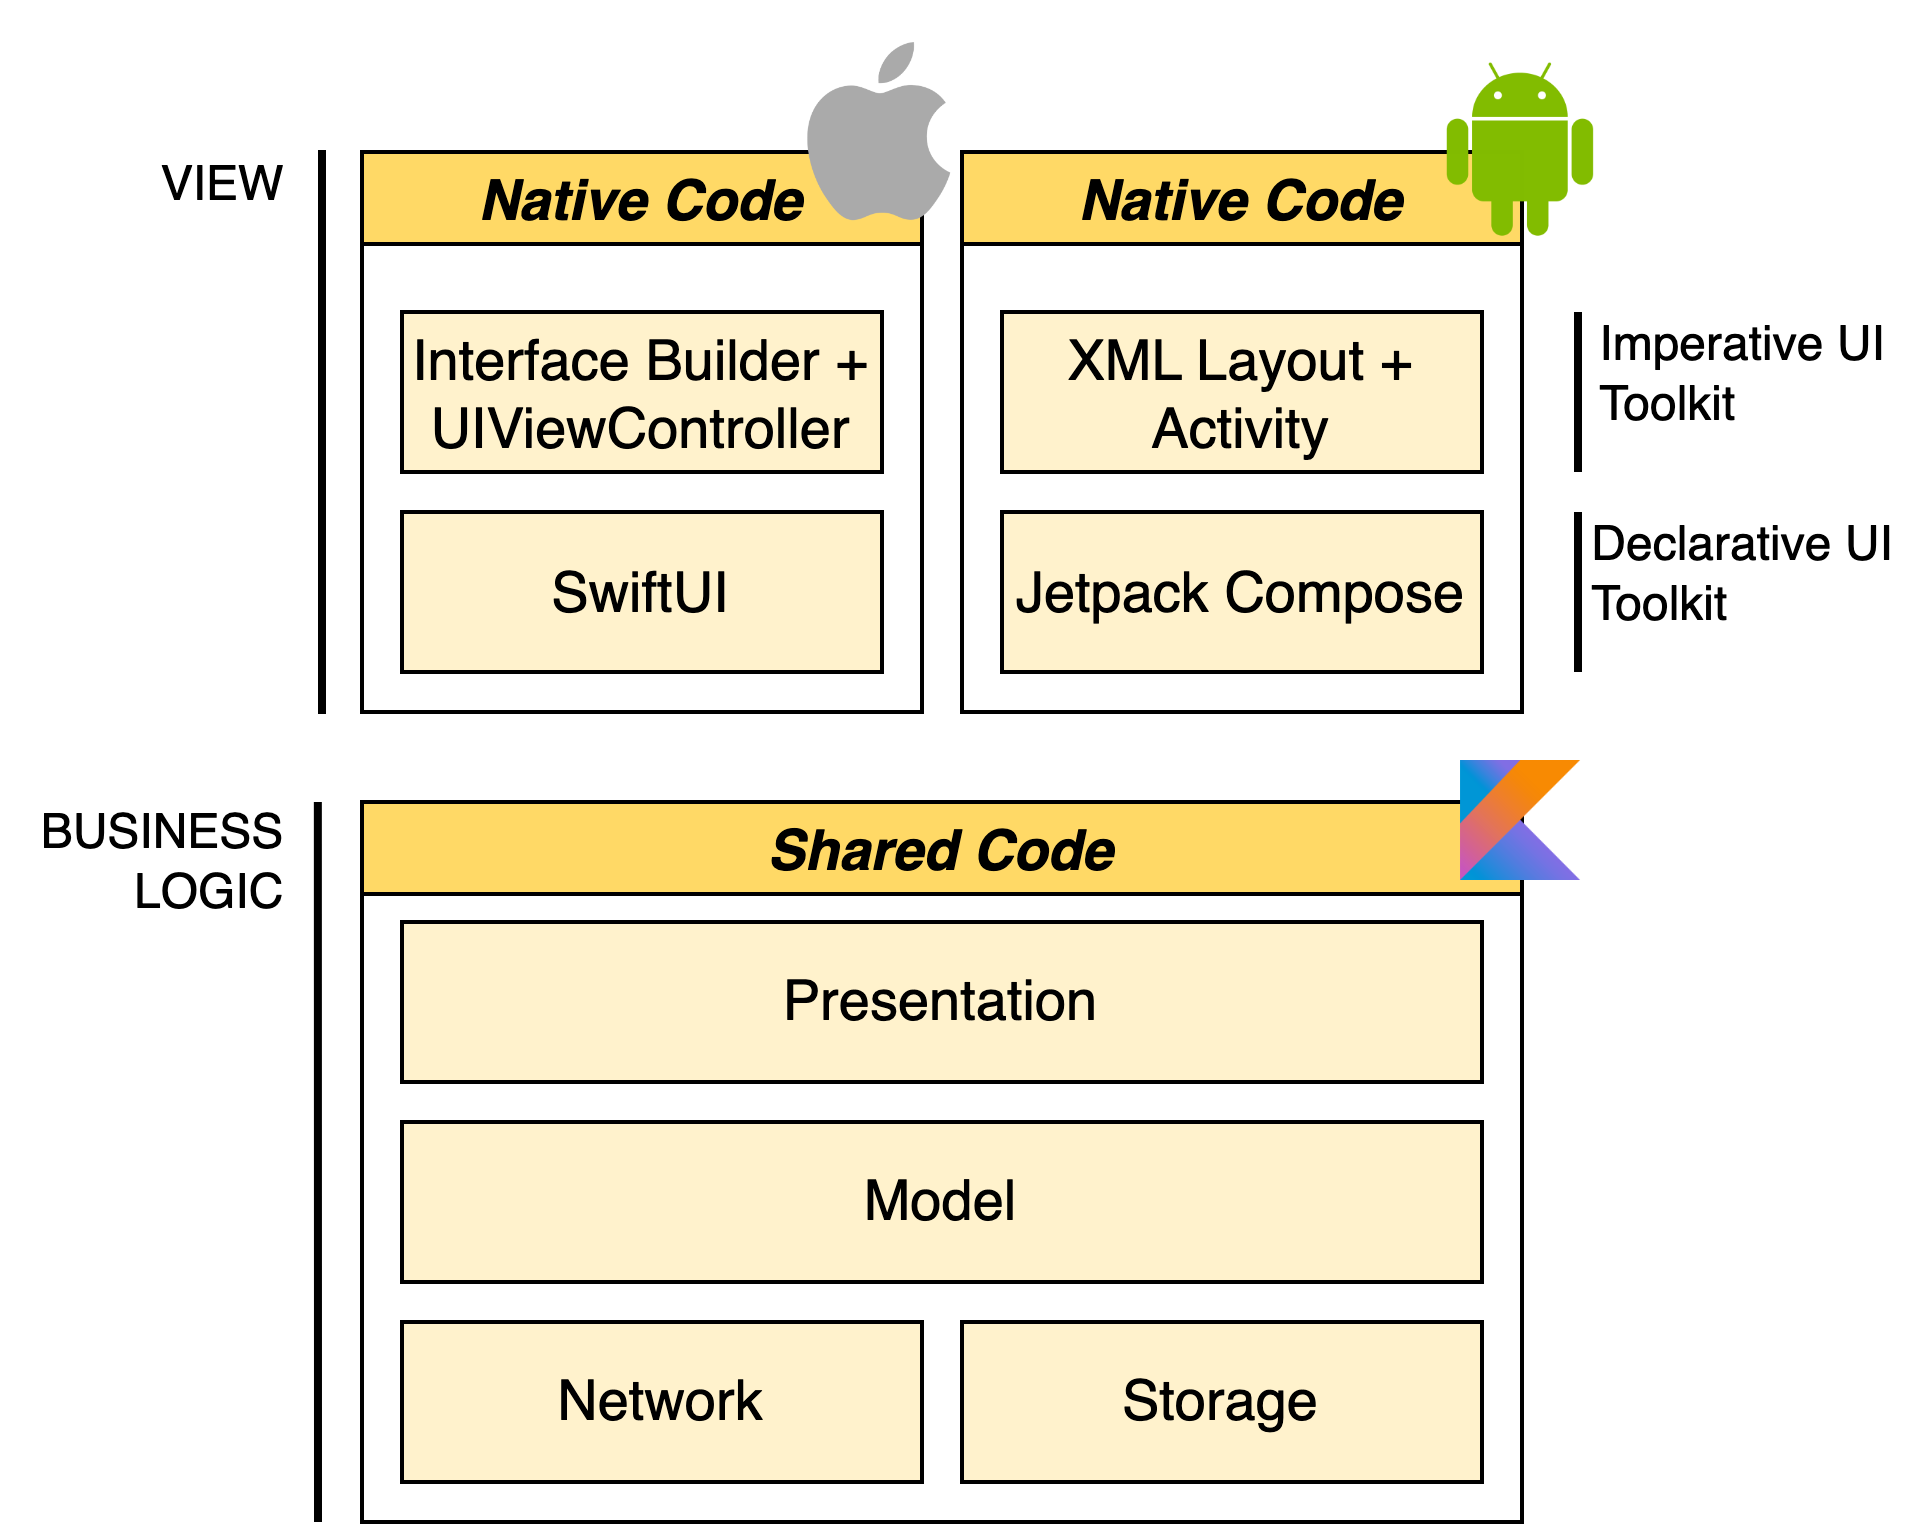
\includegraphics[width=0.73\textwidth]{img/stack_kmm.png}
    \caption{Stack architetturale Kotlin Multiplatform Mobile}
    \label{stackKMM}
\end{figure}

KMM consiste in un caso d'uso specifico (e il più diffuso) del framework Kotlin MultiPlatform (KMP),
il quale permette di sviluppare il codice in modo agnostico rispetto le piattaforme target e di condividerlo tra loro. 
Il framework KMM per poter svolgere la sua principale funzionalità di condivisione di codice si basa fortemente sui seguenti compilatori inclusi nell'ecosistema Kotlin~\cite{nagy2022simplifying}:

\begin{itemize}
    \item \textbf{Kotlin/JVM} - Utilizzato per la piattaforma Android, permette di compilare codice Kotlin in bytecode Java (\textit{.class}), il quale può essere eseguito direttamente sulla JVM. Nel caso di Android è necessario un ulteriore passaggio per tradurre il bytecode Java in bytecode Dalvik (\textit{.dex}).

    \item \textbf{Kotlin/Native} - Utilizzato per la piattaforma iOS. A differenza del compilatore Kotlin/JVM, il compilatore Kotlin/Native è progettato per quelle situazioni dove non è possibile/non si vuole avere una VM, come nel caso dei dispositivi embedded e della piattaforma iOS. Per fare ciò include un backend basato su \textit{Low Level Virtual Machine} (LLVM)\footnote{\href{https://llvm.org/}{https://llvm.org/}} in grado di compilare il codice Kotlin in binari nativi che possono essere eseguiti senza VM\cite{nagy2022simplifying}. Le piattaforme supportate da Kotlin/Native attualmente sono macOS, iOS, tvOS, watchOS, Linux, Windows (MinGW) e Android NDK\footnote{\href{https://kotlinlang.org/docs/native-overview.html\#target-platforms}{https://kotlinlang.org/docs/native-overview.html\#target-platforms}} e per ognuna di esse esistono differenti architetture. Nel caso di iOS le differenti architetture supportate da KMM sono \textit{Arm64}, \textit{Arm32} e \textit{x64}. Anche in questo caso sono necessarie due fasi di compilazione: (\textit{i}) il codice Kotlin viene compilato nella \textit{Rappresentazione Intermedia} (IR) LLVM e (\textit{ii}) successivamente compilato nel binario nativo.
\end{itemize}

\begin{figure}[H]
    \centering
    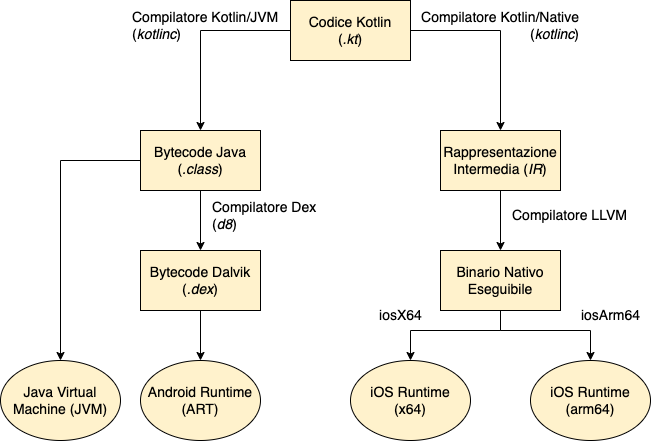
\includegraphics[width=0.82\textwidth]{img/compilatore_kotlin.png}
    \caption{Fasi di compilazione Kotlin/JVM e Kotlin/Native}
    \label{kotlin-native-compile}
\end{figure}

\subsection{Struttura Applicazione KMM}
Un'applicazione sviluppata con KMM segue lo stack definito dalla condivisione della business logic e la separazione della UX/UI (fig. \ref{stackKMM}). 
Il modulo \textit{shared} contiene tutta la business logic condivisa, 
la quale può essere sviluppata tramite l'utilizzo di librerie con supporto nativo al framework KMM, 
cioè librerie che forniscono già al loro interno specifiche implementazioni per le diverse piattaforme target, 
oppure tramite l'utilizzo del meccanismo \textit{expect/actual}.

Nel caso di utilizzo del meccanismo expect/actual è necessario definire le funzionalità nel modulo \textit{commonMain} e fornire le implementazioni per le specifiche piattaforme nei relativi moduli \textit{androidMain} e \textit{iosMain}. 
Gli stessi concetti vengono applicati per la struttura dei moduli di test: \textit{commonTest}, \textit{androidTest} e \textit{iosTest}. 
I moduli UX/UI delle relative piattaforme includono il codice condiviso come dipendenza di progetto, 
in particolare come dipendenza Gradle (\textit{aar}\footnote{Android Archive}) per Android e come dipendenza CocoaPods (Pod) per iOS.

\begin{figure}[H]
    \centering
    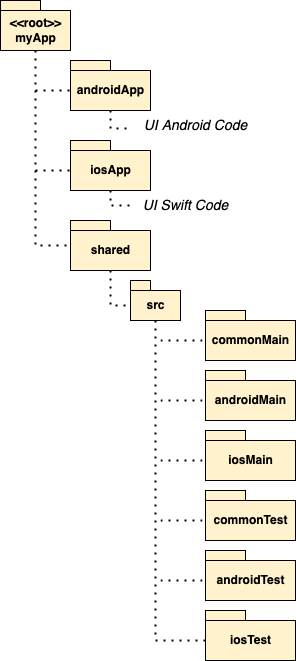
\includegraphics[width=0.55\textwidth]{img/struttura_app_kmm.png}
    \caption{Struttura dei moduli di una applicazione KMM}
\end{figure}

\subsection{Expect/Actual}
Quando si sviluppa codice condiviso è spesso necessario definire come determinate funzionalità debbano essere implementate sulla specifica piattaforma target per utilizzare i relativi SDK\footnote{Software Development Kit}. 
Il framework KMM fornisce il meccanismo \textit{expect/actual} per assolvere a questo compito in modo del tutto analogo al design pattern \textit{Template Method}~\cite{gamma1994design}:

\begin{itemize}
    \item \textbf{Expect} - Astrazione della funzionalità necessaria. Tramite la keywork \textit{expect} si definisce lo scheletro astraendo dalla specifica implementazione.
    
    \item \textbf{Actual} - Implementazione specifica per una determinata piattaforma. Tramite la keywork \textit{actual} si definisce l'implementazione, reificando l'astrazione definita tramite il concetto di \textit{expect}.
\end{itemize}

Il seguente codice\footnote{\href{https://github.com/paganellif/DevOps-per-applicazioni-mobile-un-caso-di-studio-industriale/tree/3-applicazioni-multipiattaforma/kmm-example/shared}{https://github.com/paganellif/DevOps-per-applicazioni-mobile-un-caso-di-studio-industriale/tree/3-applicazioni-multipiattaforma/kmm-example/shared}} mostra un esempio elementare d'utilizzo del meccanismo descritto:

\begin{listing}[H]
    \inputminted{kotlin}{code/expect-actual.kt}
    \caption{Esempio di applicazione expect/actual per ottenere informazioni sulla piattaforma}
\end{listing}

I seguenti screenshot, 
catturati tramite l'esecuzione degli appositi emulatori delle piattaforme target, 
mostrano l'efficacia del meccanismo expect/actual: 
l'applicazione è stata compilata utilizzando le differenti implementazioni in modo corretto.

%\newpage
\begin{multicols}{2}
    \begin{figure}[H]
        \centering
        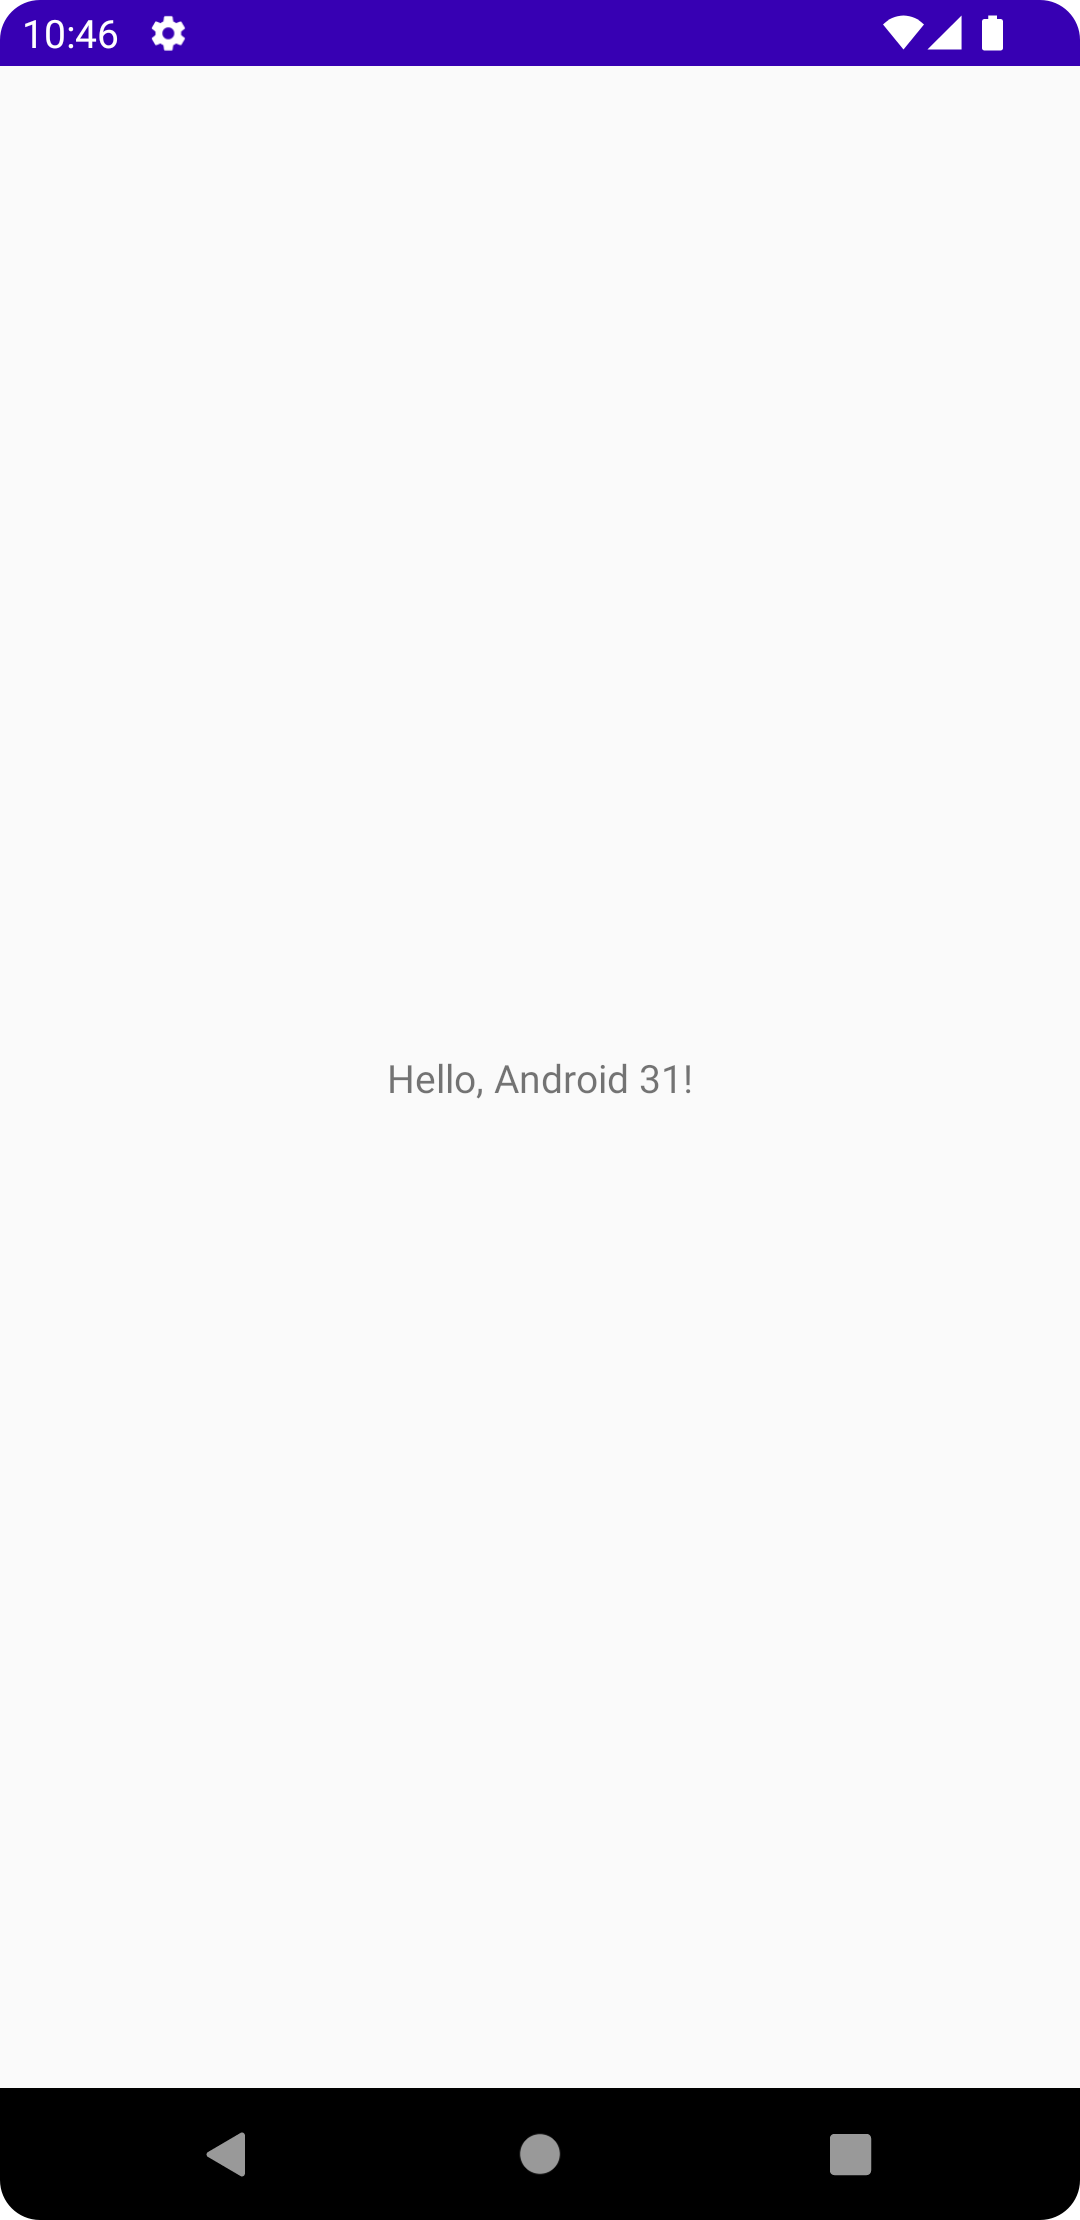
\includegraphics[width=0.35\textwidth]{img/kmm_example_android.png}
        \caption{Esempio expect/actual in esecuzione sulla piattaforma Android}
        \label{expect-actual-android}
    \end{figure}

    \begin{figure}[H]
        \centering
        
\includegraphics[width=0.33\textwidth]{img/kmm_example_ios_dark.png}
        \caption{Esempio expect/actual in esecuzione sulla piattaforma iOS}
        \label{expect-actual-ios}
    \end{figure}
\end{multicols}

\subsection{KMM Gradle Plugins}
Gli strumenti di build automation permettono la gestione di tutti quei task riguardanti la compilazione del codice. 
Gradle rappresenta il tool di build automation ufficiale Android ed è possibile sviluppare delle estensioni, 
chiamate \textit{plugins}, 
per aggiungere task custom allo strumento. 
E' proprio tramite questo meccanismo che KMM permette l'esecuzione dei task relativi allo sviluppo di applicazioni mobile multipiattaforma.

Lo strumento di build automation Gradle e i relativi plugins utilizzati vengono configurati tramite specifici file locati insieme ai sorgenti del progetto. 
Il seguente codice\footnote{\href{https://github.com/paganellif/DevOps-per-applicazioni-mobile-un-caso-di-studio-industriale/blob/3-applicazioni-multipiattaforma/kmm-example/shared/build.gradle.kts}{https://github.com/paganellif/DevOps-per-applicazioni-mobile-un-caso-di-studio-industriale/blob/3-applicazioni-multipiattaforma/kmm-example/shared/build.gradle.kts}} mostra come è possibile configurare il modulo condiviso tramite l'apposito file definendo le specifiche dipendenze e gli specifici task per le piattaforme target:

\begin{listing}[H]
\inputminted{kotlin}{code/build.gradle.kts}
\caption{Definizione utilizzo Plugin Gradle KMM nel file \textit{build.gradle.kts} del modulo condiviso (Kotlin)}
\end{listing}

Il plugin Gradle KMM fornisce uno specifico DSL per definire e configurare i task necessari a compilare il codice condiviso per le relative piattaforme target\footnote{\href{https://kotlinlang.org/docs/multiplatform-dsl-reference.html}{https://kotlinlang.org/docs/multiplatform-dsl-reference.html}} ma permette anche l'esecuzione di un insieme di task predefiniti,
classificati nelle seguenti tipologie:

\begin{itemize}
    \item \textbf{Build} - Tasks per compilazione e linking.
    
    \item \textbf{CocoaPods} - Tasks per la gestione delle dipendenze Swift/Objective-C.
    
    \item \textbf{Interop} - Tasks relativi all'utilizzo del \textit{commonizer}\footnote{\href{https://github.com/JetBrains/kotlin/tree/master/native/commonizer}{https://github.com/JetBrains/kotlin/tree/master/native/commonizer}}.
    
    \item \textbf{Verification tasks} - Tasks per l'esecuzione dei test.
\end{itemize}

\section{Fastlane}
\label{fastlane-sec}
Nonostante vi sia la necessità di utilizzare diversi strumenti di build automation per l'esecuzione dei task di sviluppo delle due differenti piattaforme Android e iOS,
il processo di sviluppo e le fasi che lo compongono sono comuni,
indipendentemente dalla piattaforma target. 
Come descritto nei capitoli precedenti, 
lo sviluppatore deve essere in grado non solo di eseguire task strettamente correlati alla fase di sviluppo ma anche di eseguire tutti quei task che riguardano il testing, 
la stabilizzazione e il rilascio di un'applicazione.

Tra gli strumenti open-source dedicati allo sviluppo di applicazioni multipiattaforma uno dei più popolari è sicuramente Fastlane\footnote{\href{7https://github.com/fastlane/fastlane}{7https://github.com/fastlane/fastlane}}. 
Il punto di forza di questo tool è il supporto a tutte le fasi del processo di sviluppo di applicazioni mobile per entrambe le piattaforme Android e iOS,
il quale pone lo sviluppatore nella condizione di poter operare su tutto il processo tramite un unico tool.

I task delle varie fasi del processo definiscono il comportamento di Fastlane e devono essere descritti negli appositi file di configurazione,
in particolare \textit{Fastfile} e \textit{Appfile},
utilizzando due concetti principali:

\begin{itemize}
    \item \textbf{Action} - Elaborazione predefinita e configurabile tramite passaggio di parametri, la quale rappresenta il task che deve essere eseguito.
    
    \item \textbf{Lane} - Insieme di action definito dall'utente per descrivere elaborazioni complesse, ovvero task composti da più sotto-task.
\end{itemize}

Il seguente codice\footnote{\href{https://github.com/paganellif/DevOps-per-applicazioni-mobile-un-caso-di-studio-industriale/blob/3-applicazioni-multipiattaforma/fastlane/fastlane/Fastfile}{https://github.com/paganellif/DevOps-per-applicazioni-mobile-un-caso-di-studio-industriale/blob/3-applicazioni-multipiattaforma/fastlane/fastlane/Fastfile}} rappresenta un esempio di lane Fastlane per il rilascio in versione beta di applicazioni iOS. 
Tale lane, 
chiamata \textit{beta}, 
è composta da quattro action rispettivamente per: 
(\textit{i}) inizializzare l'ambiente per connettersi ai servizi cloud Apple e scaricare tutto il necessario per la fase di firma del codice, 
(\textit{ii}) compilazione del codice Swift e creazione del pacchetto \textit{ipa} contenente l'applicazione iOS, 
(\textit{iii}) pubblicazione in versione beta su Testflight e 
(\textit{iv}) invio della notifica dell'avvenuta pubblicazione su un canale Slack dedicato.

\begin{listing}[H]
    \inputminted{ruby}{code/4-fastlane}
    \caption{Esempio di definizione di una lane Fastlane per il rilascio in versione beta di applicazioni iOS}
\end{listing}